% !TeX root = ../index.tex

\section{Bestandteile der Applikationsschicht}

Die Aufgaben der Anwendungsschicht sind es, die von den Sensoren gesammelten Daten zu speichern und auf ihnen aufbauend die Aktoren zu steuern.
Zu diesem Zweck wird die Low-Code/No-Code Plattform Node-RED eingesetzt. Die Plattform erlaubt es über eine einfache, grafische Benutzeroberfläche Programmabläufe zu gestalten und bietet viele vorgefertigte Integrationen zu Softwarelösungen, welche im \gls{iot} beliebt sind.
Beispiele zu vorgefertigten Integrationen sind MQTT und die Time-Series-Datenbank InfluxDB.
Letztere wird ebenfalls im Rahmen dieser intelligenten Gartenbewässerung zur Speicherung und Auswertung der Sensorwerte eingesetzt. Eine \gls{vm} in der Computing-Infrastruktur der DHBW Mannheim dient dazu, um eine Instanz der Plattform Node-RED und eine InfluxDB darauf zu installieren.

In der Node-RED-Umgebung sind die folgenden Anwendungsszenarien umgesetzt: Speicherung der Sensordaten, Steuerung der Pumpe, Steuerung der Markise und die Interaktion mit dem Nutzer über einen Bot des Messenger-Dienstes Telegram.

Die Logik zur Speicherung der Sensordaten ist simpel. 
Je ein Programmablauf in Node-RED hört auf die Topics der verschiedenen Sensorwerte, bringt die Daten in ein passendes Format und schreibt sie in die InfluxDB.
Die Steuerung von Wasserpumpe und Markise sind allerdings komplexer und werden daher im Folgenden nochmal im Detail beschrieben.

\subsection{Steuerung der Wasserpumpe}

Das System soll selbstständig in regelmäßigen Abständen überprüfen, ob die Bodenfeuchtigkeit unter 25\% liegt.
Ist dies der Fall und ist für die nächsten 24 Stunden kein Niederschlag vorhergesagt, so soll die Pumpe aktiviert werden.

Die Pumpe soll für zwei Minuten laufen, um die Felder zu bewässern, und anschließend wieder deaktiviert werden. Damit das Wasser Zeit zum Versickern hat, soll die Prüfschleife für fünf Minuten nach Aktivieren der Pumpe ausgesetzt werden.

\begin{figure}[h]
  \centering
  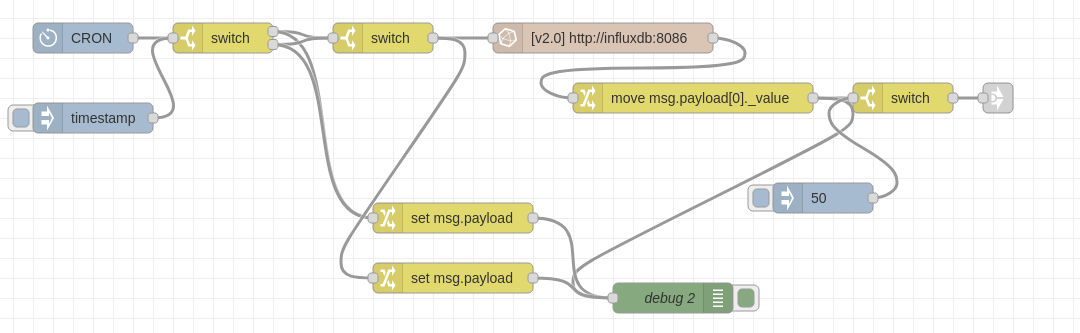
\includegraphics[width=\textwidth]{pump-activation.png}
  \caption{Überprüfungslogik für die Wasserpumpe in Node-RED}\label{fig:pump-activation}
\end{figure}

Abb. \ref{fig:pump-activation} zeigt einen Screenshot der Überprüfungslogik für die Pumpe in Node-RED.
Der Workflow wird jede Minute von dem CRON-Trigger gestartet und überprüft zunächst, ob ein globales Flag gesetzt ist, welches die Überprüfung aussetzten würde.
Darauffolgend wird kontrolliert, ob für die nächsten 24 Stunden Niederschlag vorhergesagt ist.
Die Wetterdaten hierzu werden in einem separaten Workflow regelmäßig von der öffentlichen Programmierschnittstelle des Deutschen Wetterdienstes geladen und in einer globalen Variable gespeichert.

Falls kein Niederschlag vorhergesagt ist, wird der durchschnittliche Bodenfeuchtigkeitswert der letzten fünf Minuten aus der InfluxDB ermittelt.
Liegt dieser Wert unter 25\%, wird die Steuerungslogik für die Pumpe in einem Sub-Workflow ausgeführt.
Dieser Sub-Workflow ist in Abb. \ref{fig:pump-control} dargestellt.

\begin{figure}[h]
  \centering
  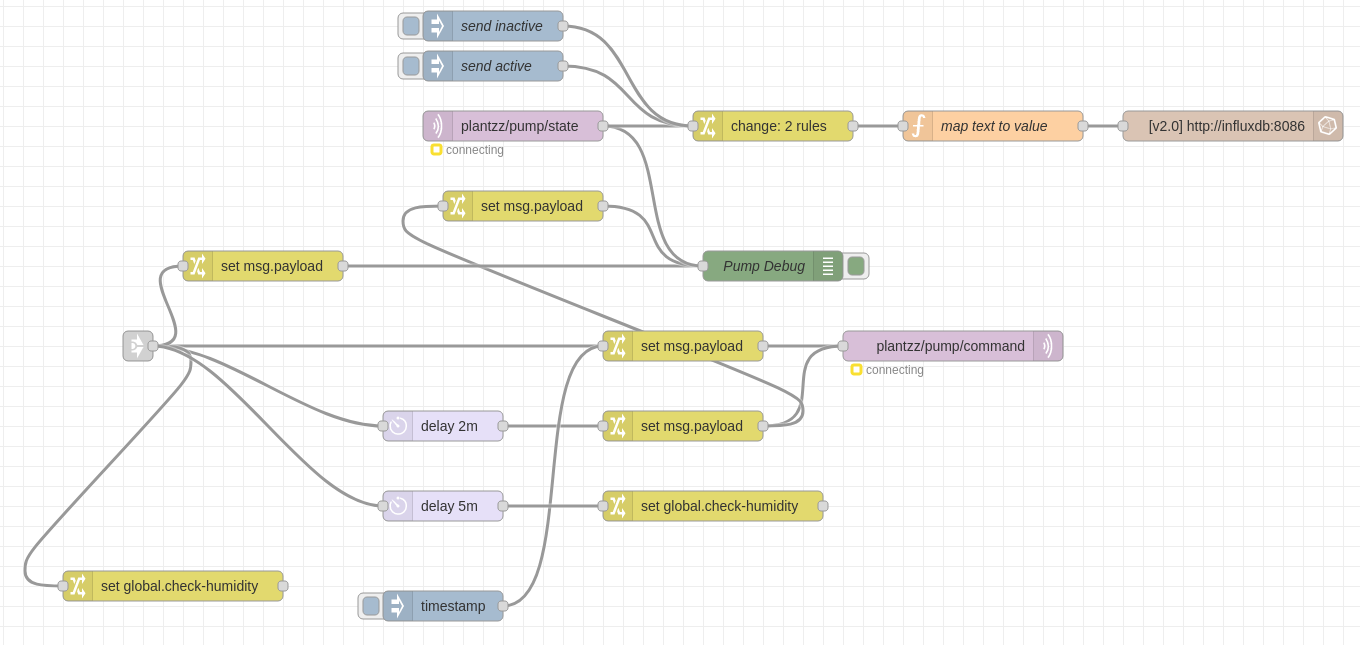
\includegraphics[width=\textwidth]{pump-control.png}
  \caption{Steuerungslogik für die Wasserpumpe in Node-RED}\label{fig:pump-control}
\end{figure}

Beim Starten der Steuerungslogik wird unmittelbar eine Nachricht mit dem Aktivierungskommando in dem MQTT-Topic der Pumpensteuerung veröffentlicht.
Zudem wird das globale Flag gesetzt, welches die die Überprüfungslogik deaktiviert.
Nach einer Verzögerung von zwei Minuten wird das Deaktivierungskommando veröffentlicht und nach fünf Minuten wird das Flag zur Deaktivierung der Überprüfungslogik wieder zurückgesetzt.

\subsection{Steuerung der Markise}

Neben der Wasserregelung soll das System fähig sein selbstständig zu überprüfen, ob eine Beschattung durch eine Markise momentan benötigt wird. Um  das Ein- und Ausfahren dieser Markise automatisch zu steuern werden einige Umwelteinflüsse überprüft. Die Markise ist im Allgemeinen von der Helligkeit abhängig. Weitere Faktoren, die ebenfalls zur Steuerung der Markise mit einbezogen werden sind außerdem die Windgeschwindigkeit, die aus Wetterdaten entnommen wird, und die Umgebungstemperatur. 
Die folgende Abb. \ref{fig:canvas-activation} zeigt den entsprechenden Ablauf in Node-RED.

\begin{figure}[h]
  \centering
  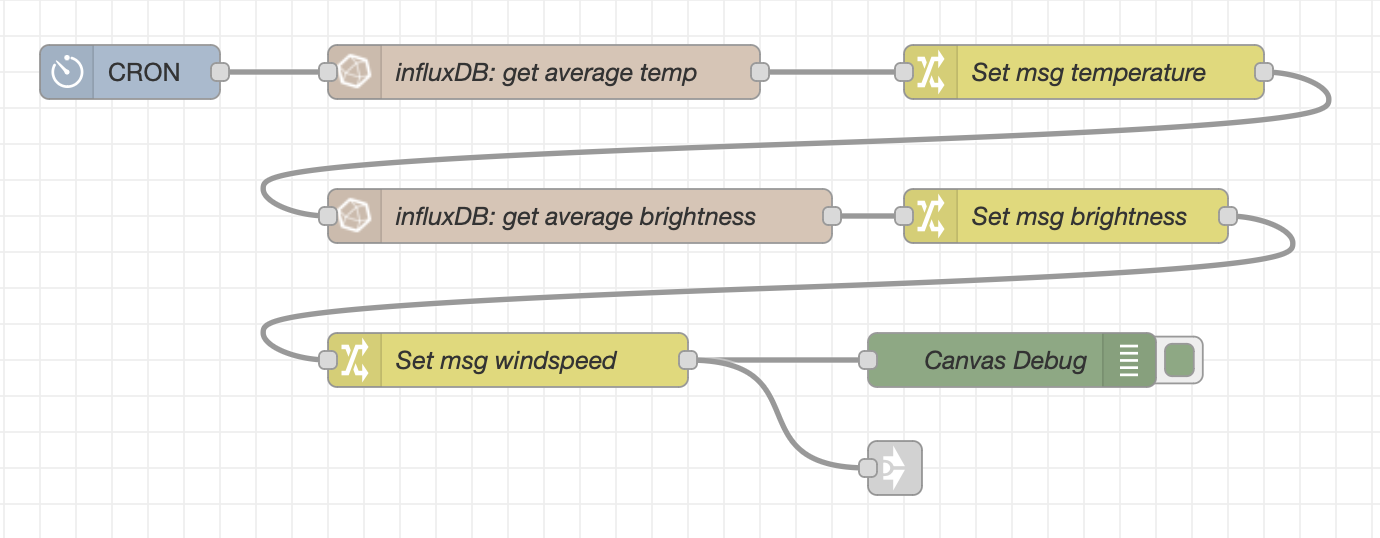
\includegraphics[width=\textwidth]{canvas-activation.png}
  \caption{Überprüfungslogik für die Markise in Node-RED}\label{fig:canvas-activation}
\end{figure}

Der Workflow startet, wie auch bei der Pumpensteuerung, mit einem CRON-Trigger einmal pro Minute. Damit die Markise ausfährt werden hintereinander die Werte für die drei Kriterien ermittelt. 

Wenn der Durschnitt der Umgebungstemperatur in den letzten fünf Minuten über 20° Celsius liegt, ist der erste Check bestanden. Diese Grenze wurde eingeführt, da eine Beschattung im Sommer beziehungsweise bei hohen Temperaturen hilft, damit die Pflanzen nicht austrocken. Bei kälteren Temperaturen würde eine Beschattung wertvolle Sonnenstrahlen von den Pflanzen abhalten. Die zweite Überprüfung betrifft die Helligkeit, für welche ebenfalls der Durschnittswert der letzen fünf Minuten ausschlaggebend ist. Wenn dieser Wert über 15000 Lux liegt ist ein weiterer Kontrollpunkt überschritten. Der letzte Punkt, der noch überprüft wird, dient der Unversehrtheit der Markise. Die Markise darf nur ausfahren wenn die Windgeschwindigkeit von 14 m/s nicht überschritten ist.

Sind die drei Werte zur Überprüfung der Bedingungen ermittelt worden, so wird der Sub-Workflow zur Markisensteuerung angestoßen. Abb. \ref{fig:canvas-control} zeigt einen Ausschnitt aus Node-RED bezüglich des Sub-Workflows.

\begin{figure}[h]
  \centering
  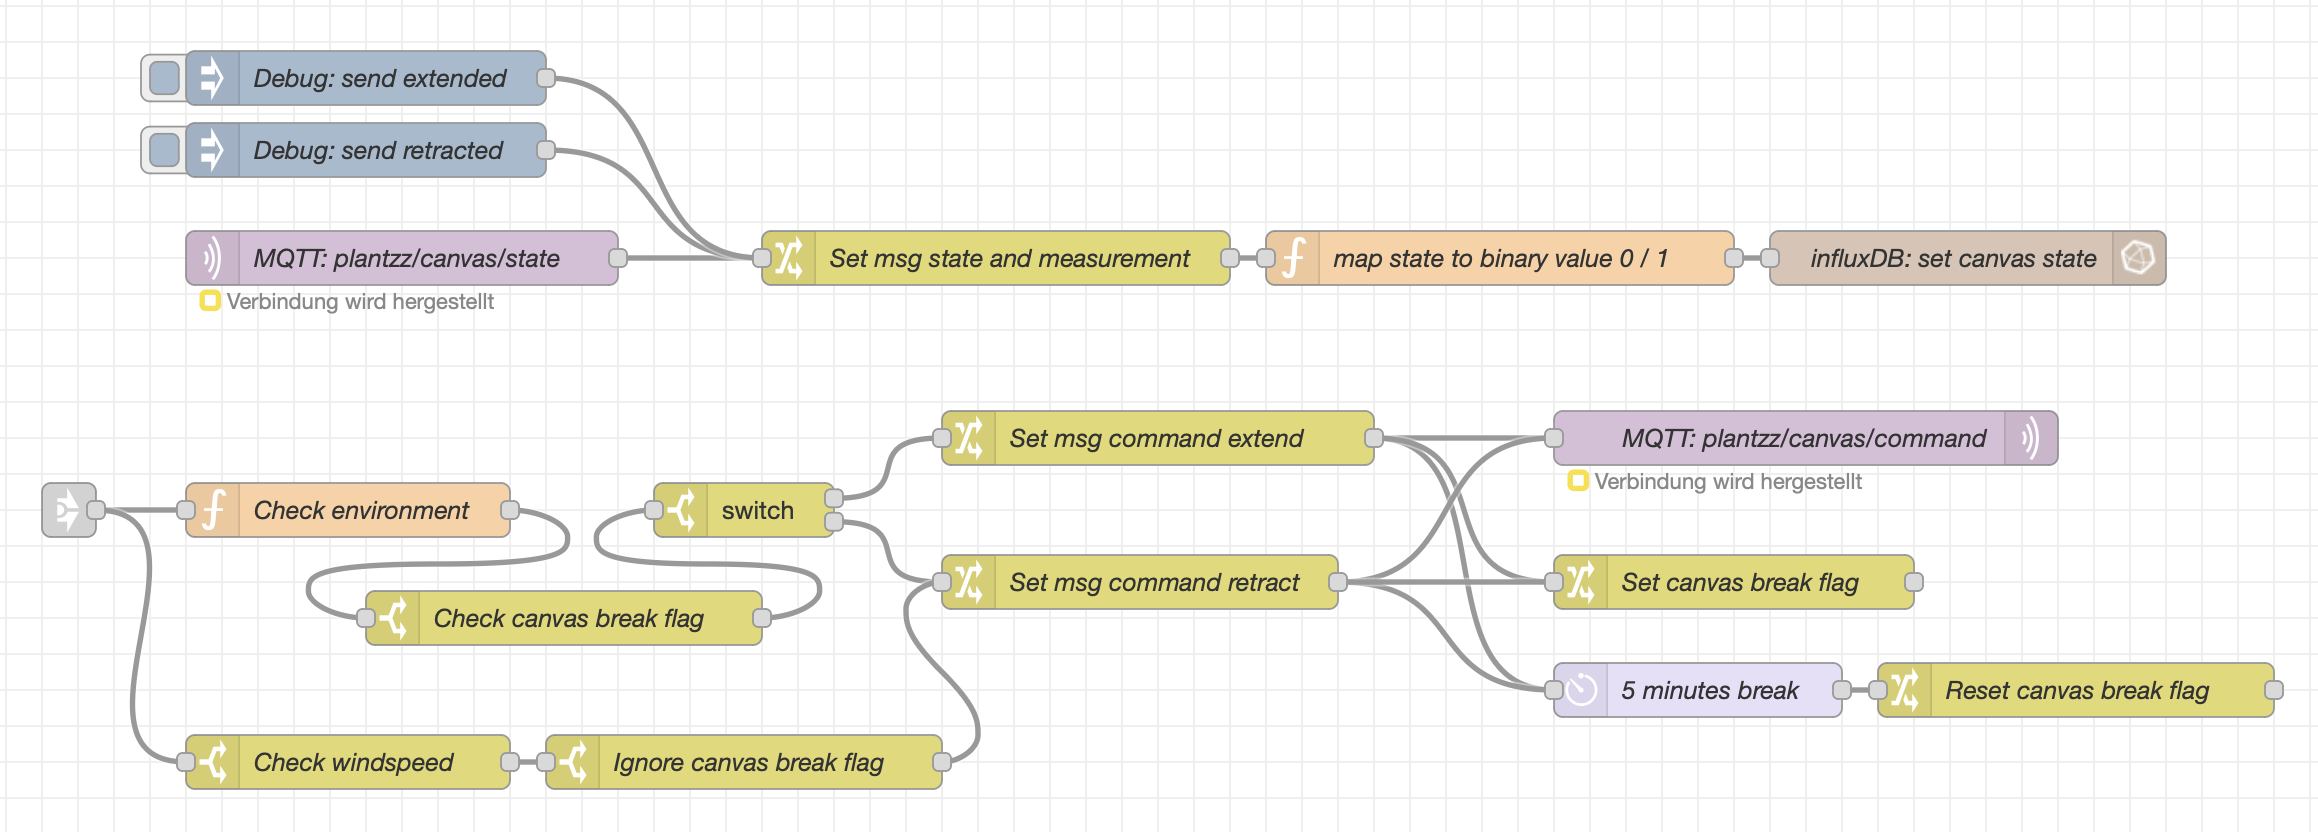
\includegraphics[width=\textwidth]{canvas-control.png}
  \caption{Steuerungslogik für die Markise in Node-RED}\label{fig:canvas-control}
\end{figure}

In der Funktion "Check environment" werden zunächst die bereits beschriebenen Checks durchgeführt. Danach wird abhängig vom Ergebnis der drei Überprüfungen entweder die Markise ein- oder ausgefahren.
Sobald der Befehl zum Ein- oder Ausfahren der Markise erteilt wurde, wird gleichzeitig die Freigabe zum erneuten Überprüfen der Markisensteuerung für fünf Minuten deaktiviert, um ein andauerndes Ein- und Ausfahren bei sich leicht ändernden Bedingungen im Grenzbereich zu verhindern. Parallel dazu wird die Windgeschwindigkeit als einzelnes Kriterium gesetzt, um die Markise bei Überschreiten des Grenzwerts sofort einfahren zu lassen, auch wenn das Flag zur Pause gesetzt ist.

\subsection{Einbindung eines Telegram Chat-Bots}

Zur Interaktion mit dem Nutzer wurde in der Applikationsschicht außerdem ein Telegram Chat-Bot implementiert. Über den Chat-Bot sind verschiedene Funktionen umsetzbar. Im Rahmen dieser Laborarbeit wurde ein Frostschutz umgesetzt: Sinkt die Bodentemperatur unter den Grenzwert von 3° Celsius, so erhält der Nutzer über den Messenger Telegram eine Warnung, dass der Boden droht zu gefrieren. Der Nutzer kann dadurch weitere Maßnahmen zum Schutz der Pflanzen einleiten. Die Definition dieser Funktion findet ebenfalls auf der Plattform Node-RED statt.

Neben der Frostschutzfunktion können weitere Chat-Funktionen in Node-RED ausgestaltet werden. Zum Beispiel könnte der Nutzer über das Senden von gewissen Schlüsselwörtern das Ein- und Ausfahren der Markise manuell anstoßen. Die Umsetzung weiterer Chat-Funktionen wurde allerdings in der Laborarbeit nicht näher behandelt.